\documentclass[conference]{IEEEtran}
\IEEEoverridecommandlockouts

\usepackage{cite}
\usepackage{amsmath,amssymb,amsfonts}
\usepackage{graphicx}
\usepackage{booktabs}
\usepackage{url}
\usepackage[hidelinks]{hyperref}

\graphicspath{{figures/}}

\def\BibTeX{{\rm B\kern-.05em{\sc i\kern-.025em b}\kern-.08em
    T\kern-.1667em\lower.7ex\hbox{E}\kern-.125emX}}

\begin{document}
\bstctlcite{IEEEexample:BSTcontrol}

\title{Do Register Tokens Regularize Vision Transformers Under Data Scarcity?\\
A Controlled 24-Run Empirical Ablation on Low-Data CIFAR-100}

\author{
\IEEEauthorblockN{Shahin Alakparov, Gulnisa Abdurahmanli, Narmina Ibrahimova, Emil Ahmedli, and Rufet Dosteliyev}
\IEEEauthorblockA{\textit{Deep Learning, Cohort 1 2026}\\
Track 1: Pure Research}
}

\maketitle

\begin{abstract}
Register tokens were originally introduced to remove high-norm attention artifacts in large vision transformers trained on massive datasets. Their behavior in data-scarce regimes, where a compact model is fine-tuned on limited samples, remains largely uncharacterized. In this work, we investigate whether register tokens provide structural regularization under data scarcity. We conduct a fully paired, controlled empirical ablation across 24 training runs on CIFAR-100 subsets, evaluating ViT-Tiny across four register allocations ($K \in \{0, 1, 4, 8\}$) and two data budget regimes (100 and 300 images per class, with three random seeds per arm). On the untouched 10{,}000-image test set at 100 images per class, no register configuration outperforms the register-free control ($75.19 \pm 0.24\%$). While $K=4$ exhibits an apparent regularization signal on the small validation split by lowering validation loss ($\Delta = -0.034$, $p = 0.024$) and narrowing the generalization gap, this effect fails to transfer to held-out test performance ($\Delta = +0.002$, $p = 0.823$). To test whether this null result stems from extreme data starvation, we scale the training budget threefold to 300 images per class. While baseline test accuracy surges by $+6.14\%$ to $81.33 \pm 0.37\%$, register tokens continue to yield no statistically significant advantage ($81.23 \pm 0.19\%$ for $K=1$, $81.23 \pm 0.18\%$ for $K=4$, and $81.02 \pm 0.45\%$ for $K=8$). Furthermore, layer-wise attention entropy and patch-norm outlier rates confirm the absence of attention-sink suppression. We conclude that register tokens do not regularize vision transformers under data scarcity, and that mechanisms observed at foundation scale do not automatically generalize to compact models in low-data regimes.
\end{abstract}


\begin{IEEEkeywords}
vision transformers, register tokens, attention entropy, generalization gap, low-data regime, negative results
\end{IEEEkeywords}

\section{Introduction}

Vision transformers develop a peculiar failure of interpretability at scale.
Darcet \textit{et al.}~\cite{darcet2024registers} observed that in large
supervised and self-supervised ViTs a small number of patch tokens acquire
anomalously large activation norms, and that the \texttt{[CLS]} token routes a
disproportionate share of its attention to them. These tokens sit in
low-information image regions, carry global rather than local content, and make
attention maps unusable as saliency evidence. The proposed remedy is
architectural and cheap: prepend $K$ learnable \emph{register} tokens to the
input sequence, discard them at the output, and let the model use them as the
scratch space it was previously carving out of the image itself. At scale this
works---the artifacts disappear and downstream performance is unaffected or
mildly improved.

The mechanism reported in that work is a \emph{cleanup} effect, demonstrated in
a regime where the model has far more data than it can overfit. This leaves an
obvious question unanswered. If registers absorb capacity that the model would
otherwise spend on memorising the training set, they should behave like a
regularizer, and the place to look for a regularizer is the regime where
overfitting is the binding constraint: a small model trained on scarce data.

We therefore ask a narrow, falsifiable question:

\begin{quote}
\textit{When a ViT is starved of data, do register tokens reduce the
generalization gap, and does any such reduction transfer to held-out
performance?}
\end{quote}

We test three hypotheses drawn from the original mechanism:

\begin{itemize}
\item[\textbf{H1}] \textbf{Structural regularization.} Registers reduce the
generalization gap $\Delta\mathcal{L} = \mathcal{L}_{\mathrm{val}} -
\mathcal{L}_{\mathrm{train}}$.
\item[\textbf{H2}] \textbf{Capacity dilution.} At an embedding width of
$d = 192$, a large $K$ consumes representational capacity and degrades
accuracy, producing a non-monotonic response in $K$.
\item[\textbf{H3}] \textbf{Entropy collapse prevention.} Registers prevent the
layer-wise collapse of attention entropy that accompanies artifact formation.
\end{itemize}

Our contributions are:

\begin{enumerate}
\item A fully paired $4 \times 3$ ablation ($K \in \{0,1,4,8\}$, seeds
\texttt{42}, \texttt{1337}, \texttt{3407}) on a strict 100-images-per-class
CIFAR-100 subset, with every hyperparameter, data split and schedule held fixed
across arms, so that $K$ is the only manipulated variable.
\item A statistical treatment appropriate to $n = 3$: differences are formed
\emph{within} a seed before reduction, which removes the seed variance that
otherwise dominates the treatment effect at this sample size.
\item A separation of validation-measured from test-measured effects. This
separation is what turns an apparently positive result into a negative one: the
gap reduction predicted by H1 is present and consistent on the validation
split, and absent on the held-out test split.
\item A negative result reported as such, with the mechanism-level evidence
(layer-wise entropy, patch-norm outlier rates, training-loss equality) that
distinguishes ``registers did nothing'' from ``registers helped somewhere we
could not measure''.
\end{enumerate}

We find no configuration that beats the register-free control on held-out
accuracy. H1 is not supported on held-out data, H2 is supported at $K=8$, and
H3 is not supported. Section~\ref{sec:discussion} argues that the most likely
reason is a regime mismatch rather than a refutation of
\cite{darcet2024registers}: our backbone is ImageNet-pretrained, the registers
are randomly initialised into it, and 50 epochs over 9{,}000 images is a short
window in which to learn a new routing behaviour from scratch.

\section{Related Work}

\subsection{Vision transformers and low-data training}

The ViT~\cite{dosovitskiy2021vit} replaces convolutional inductive bias with
global self-attention over patch embeddings, and pays for it with a strong data
appetite. DeiT~\cite{touvron2021deit} showed that heavy augmentation and
distillation recover competitive ImageNet accuracy without external data, and
the systematic study of Steiner \textit{et al.}~\cite{steiner2022howtotrain}
mapped how augmentation and regularization trade against dataset size for ViTs
of several widths. Both establish the setting we work in: when data is scarce, a
ViT is regularization-limited rather than capacity-limited, which is exactly the
regime in which a candidate regularizer should show its effect most clearly.

\subsection{Attention artifacts and register tokens}

Darcet \textit{et al.}~\cite{darcet2024registers} identified high-norm outlier
patch tokens in DINOv2~\cite{oquab2024dinov2} and OpenCLIP, showed that these
tokens are recycled by the network as global scratch space, and removed them by
appending learnable register tokens. The same phenomenon has a language-model
analogue: attention sinks~\cite{xiao2024streamingllm}, where a small number of
positions absorb attention mass that the model has nowhere else to put, and
massive activations~\cite{sun2024massive}, which characterises the outlier
coordinates involved. The common thread is that the artifact is a symptom of a
missing degree of freedom, and that supplying that degree of freedom explicitly
removes the symptom.

What none of this work reports is an effect on \emph{generalization}. In
\cite{darcet2024registers} the register variants match or slightly exceed their
baselines, and the argument is made on interpretability and dense-prediction
grounds. The claim that registers reduce overfitting is a hypothesis that the
original evidence neither establishes nor rules out, and it is the hypothesis we
test here.

\subsection{Attention entropy as a diagnostic}

Attention distributions are probability vectors, so their Shannon entropy is a
direct, parameter-free measure of how concentrated the routing is. Artifact
formation should appear as a fall in entropy in the deeper blocks, where the
\texttt{[CLS]} token has been observed to concentrate on a few outlier
positions. We use layer-resolved entropy as the mechanism-level readout for H3,
alongside the patch-norm outlier rate that defines the artifacts in
\cite{darcet2024registers}.

\subsection{Positioning}

To our knowledge the register question has not been asked in the low-data,
small-model, ImageNet-pretrained fine-tuning regime, and it has not been asked
with a generalization-gap framing under a fixed compute budget. Our answer is
negative, and we regard reporting it as such, rather than selecting the split
on which the effect appears, as the contribution.

\section{Method}
\label{sec:method}

\subsection{Register-augmented vision transformer}

Let $x \in \mathbb{R}^{3 \times H \times W}$ be an input image, partitioned by a
$16 \times 16$ patch embedding into $N = 196$ patch tokens of width $d = 192$.
The standard ViT prepends a classification token, giving the sequence
$[\,\texttt{[CLS]}, p_1, \dots, p_N\,]$. We insert $K$ learnable register
tokens $r_1 \dots r_K \in \mathbb{R}^{d}$ between the two groups:

\begin{equation}
z^{(0)} = [\,\texttt{[CLS]},\; r_1, \dots, r_K,\; p_1, \dots, p_N\,] + E_{\mathrm{pos}},
\end{equation}

where positional embeddings $E_{\mathrm{pos}}$ are applied to the
\texttt{[CLS]} and patch positions of the pretrained backbone; registers carry
no positional embedding, as they correspond to no spatial location. The
sequence length becomes $S = 1 + K + N$. The registers participate fully in
every self-attention block and are discarded before the classification head,
which reads the \texttt{[CLS]} token only. The register block is initialised
with a truncated normal, $r_i \sim \mathcal{N}_{\mathrm{trunc}}(0, 0.02^2)$;
zero initialisation is avoided because it makes the register columns
indistinguishable and stalls their gradient.

The parameter cost is $K \cdot d$ weights, which is negligible: $K=8$ adds
1{,}536 parameters to a 5.54\,M-parameter model, a relative increase of
$2.8 \times 10^{-4}$. Any measured difference between arms is therefore
attributable to the tokens' function, not to added capacity in the usual sense.

\subsection{Diagnostic measures}

\subsubsection{Layer-wise attention entropy}
For block $l$ with attention matrix
$A^{(l)} \in \mathbb{R}^{B \times H \times S \times S}$, whose rows are
probability distributions over keys, we compute the Shannon entropy of each row
and average over batch, heads and query positions:

\begin{equation}
\bar{H}^{(l)} = -\frac{1}{BHS}\sum_{b,h,i}\sum_{j=1}^{S} A^{(l)}_{b,h,i,j}\log_2\!\big(A^{(l)}_{b,h,i,j} + \epsilon\big),
\end{equation}

with $\epsilon = 10^{-12}$. Units are bits. A concentrated, artifact-like
routing pattern lowers $\bar{H}^{(l)}$; a diffuse one raises it. Because
recent \texttt{timm} builds execute fused scaled-dot-product attention, the
$[B,H,S,S]$ matrix is never materialised in the forward pass; our hook
reconstructs the softmax weights from the block's own $Q$ and $K$ projections,
reapplying the same scaling and any $q$/$k$ normalisation, so the recovered
matrix is the one the model used.

\subsubsection{Patch-norm outlier rate}
Following the artifact definition of \cite{darcet2024registers}, we take the
block-output residual stream $h^{(l)} \in \mathbb{R}^{B \times S \times d}$,
restrict it to the spatial positions $1+K \dots S$, and compute per-sample the
fraction of patch tokens whose $\ell_2$ norm exceeds three standard deviations
above the per-sample mean:

\begin{equation}
\rho^{(l)} = \frac{1}{BN}\sum_{b}\sum_{n} \mathbf{1}\!\left[\;\lVert h^{(l)}_{b,\,K+n}\rVert_2 > \mu^{(l)}_b + 3\sigma^{(l)}_b \;\right].
\end{equation}

The offset $1+K$ matters: slicing from index 1 would count register tokens as
image patches, and registers are expected to carry large norms by design, so
the error would manufacture exactly the artifact the metric is meant to detect.

\subsubsection{Generalization gap}
The regularization hypothesis is stated on losses rather than accuracies,
because loss is the quantity the optimiser acts on:

\begin{equation}
\Delta\mathcal{L}_s = \mathcal{L}^{\mathrm{val}}_{s}(e^{\star}_s) - \mathcal{L}^{\mathrm{train}}_{s}(E),
\end{equation}

where $e^{\star}_s$ is the epoch selected for seed $s$ and $E$ is the final
epoch. The gap is formed \emph{within} a seed before any averaging. Averaging
the two losses separately and subtracting would produce the same mean but
destroy the pairing, and with it any valid dispersion estimate for the gap;
since H1 is judged on that dispersion, the ordering of operations is part of
the method rather than an implementation detail.

\subsection{Statistical treatment}

With three seeds per arm, an unpaired comparison of arm means is dominated by
seed variance: the between-seed standard deviation of validation Top-1 in the
control arm ($2.17$ pp) is an order of magnitude larger than any treatment
effect we could plausibly detect. Every comparison in this paper is therefore
paired. For metric $m$, arm $K$ and the shared seed set
$\mathcal{S} = \{42, 1337, 3407\}$ we form

\begin{equation}
\delta_s = m_s(K) - m_s(0), \qquad s \in \mathcal{S},
\end{equation}

and report $\bar{\delta}$, its sample standard deviation $\hat{\sigma}_\delta$
(with $\mathrm{ddof} = 1$), the count of seeds moving in the hypothesised
direction, and the paired statistic
$t = \bar{\delta} / (\hat{\sigma}_\delta / \sqrt{3})$ against Student's $t$ with
$\mathrm{df} = 2$. Arm-level dispersion in Table~\ref{tab:main_results} uses the
population convention ($\mathrm{ddof} = 0$), which is recorded in the emitted
summary artifact so the estimator is never ambiguous.

Two cautions apply throughout and we state them once. First,
$\mathrm{df} = 2$ gives these tests very low power; a $p$-value here is
effect-size evidence, not a confirmatory test. Second, we report fifteen paired
comparisons without multiplicity correction, so an isolated small $p$ among
them is weak evidence. Accordingly we treat the direction count---how many of
three seeds move the same way---as the primary signal and the $p$-value as
secondary.

\section{Experimental Setup}
\label{sec:setup}

\subsection{Data}

We use CIFAR-100~\cite{krizhevsky2009cifar} restricted to a strict low-data
budget. From the 50{,}000-image training split we draw a stratified subset of
100 images per class (10{,}000 images), split $90/10$ into 9{,}000 training and
1{,}000 validation images with the class proportions preserved. The full,
untouched 10{,}000-image test split is used once per run, after training, and is
never consulted for model selection. Images are bicubically resized to
$224 \times 224$ so that the pretrained patch grid and positional embeddings
apply without interpolation. Training uses random resized crop
($\mathrm{scale} \in [0.8, 1.0]$), horizontal flip and
AutoAugment~\cite{cubuk2019autoaugment} with the CIFAR-10 policy; evaluation
uses resize and centre crop only. Normalisation uses the CIFAR-100 channel
statistics.

The stratified subset is drawn under the run's own seed, so the three seeds
differ in \emph{which} 100 images per class are selected as well as in
initialisation and batch order. This makes the seed a genuine replicate of the
whole experimental pipeline rather than of initialisation alone, and it is the
main reason the between-seed dispersion is as large as it is. Within a seed the
subset, the split and the batch order are identical across all four arms, which
is what makes the paired comparison of Section~\ref{sec:results} a comparison of
$K$ and of nothing else.

\subsection{Model and training}

The backbone is \texttt{vit\_tiny\_patch16\_224} from
\texttt{timm}~\cite{wightman2019timm}: 12 blocks, 3 heads, $d = 192$,
ImageNet-pretrained, with a fresh 100-way linear head. Register tokens are
appended to this pretrained backbone and are the only randomly initialised
parameters besides the head. Total parameter counts are 5{,}543{,}716 ($K=0$)
through 5{,}545{,}252 ($K=8$).

All arms share one configuration: 50 epochs, batch size 64,
AdamW~\cite{loshchilov2019adamw} at $\eta = 5 \times 10^{-4}$ with weight decay
$0.05$, cosine decay~\cite{loshchilov2017sgdr} to $\eta_{\min} = 10^{-5}$ after
5 warmup epochs, gradient clipping at $1.0$, label smoothing
$\varepsilon = 0.1$~\cite{szegedy2016rethinking}, and automatic mixed
precision~\cite{micikevicius2018mixed} in PyTorch~\cite{paszke2019pytorch}.
Because losses are label-smoothed they
carry a constant positive floor; they are comparable across arms, which is all
we require, but not against unsmoothed values reported elsewhere. Model
selection takes the epoch with the lowest validation loss.

\subsection{The 24-run experimental matrix and budget scaling}

The study evaluates the full cross-product of $K \in \{0, 1, 4, 8\}$ across three pinned random seeds $\{42, 1337, 3407\}$ under two distinct data budget regimes, yielding 24 runs in total:
\begin{itemize}
\item \textbf{Primary Low-Data Benchmark (100 images/class):} 10{,}000 images total (9{,}000 train, 1{,}000 validation), running experiments \texttt{exp01} through \texttt{exp12}.
\item \textbf{Data Budget Scaling Extension (300 images/class):} 30{,}000 images total (27{,}000 train, 3{,}000 validation), running experiments \texttt{exp13} through \texttt{exp24} to evaluate whether empirical conclusions remain scale-invariant when data scarcity is relaxed threefold.
\end{itemize}

Each run writes to an isolated output directory keyed by its experiment ID, register count, and seed. A run is admitted only if all required artifacts (\texttt{metrics.json}, \texttt{best\_model.pth}, \texttt{last\_model.pth}, \texttt{train\_history.csv}) are generated and structurally validated. All 24 planned runs completed without failure across 8+ hours of compute on an NVIDIA A100-SXM4 GPU.

\subsection{Where the diagnostics are measured}

Attention entropy and the patch-norm outlier rate are read from the first
evaluation batch of the test pass (64 images), with the hooks disarmed
immediately afterwards to bound host memory. The test loader is unshuffled, so
this evaluates the identical 64 images in every run, ensuring paired entropy
comparisons operate on identical inputs. Section~\ref{sec:limitations} discusses
the sample bounds of this batch.

\subsection{Reporting pipeline}

Each run emits a nested \texttt{metrics.json}. An automated aggregation engine extracts
the necessary quantities from that structure (including validation loss at the selected epoch,
final training loss from the terminal record, and layer-resolved test diagnostics), reduces
them across seeds, and outputs structured summary files (\texttt{sweep\_summary.json} and
\texttt{summary.json}). Every table and figure in this paper is generated directly from these
verified artifacts via script. The table generator recomputes statistics independently from
the raw per-run records, ensuring that no metric is transcribed by hand.

\section{Results}
\label{sec:results}

\begin{table*}[t]
\centering
\caption{Register ablation on low-data CIFAR-100 (100 images/class, ViT-Tiny, 50 epochs). Mean $\pm$ population standard deviation over the three seeds \texttt{42}, \texttt{1337} and \texttt{3407}; best value per column in bold. Test metrics come from a single pass over the untouched 10{,}000-image test split. Validation loss is the value at the selected epoch and is therefore a selected minimum, not an unbiased estimate. The gap $\Delta\mathcal{L}=\mathcal{L}_{\mathrm{val}}-\mathcal{L}_{\mathrm{train}}$ is formed within each seed before averaging. Losses are label-smoothed ($\varepsilon=0.1$) cross-entropy, so they carry a constant positive floor and are comparable across arms but not against unsmoothed values.}
\label{tab:main_results}
\setlength{\tabcolsep}{5pt}
\footnotesize
\begin{tabular}{lccccc}
\toprule
\textbf{Configuration} & \textbf{Test Top-1 (\%)} & \textbf{Test Loss} & \textbf{Val Loss} & \textbf{Gap $\Delta\mathcal{L}$} & \textbf{$\bar{H}^{(12)}$ (bits)} \\
\midrule
Baseline ($K=0$) & \textbf{75.19 $\pm$ 0.24} & \textbf{1.6357 $\pm$ 0.0018} & 1.6829 $\pm$ 0.0609 & 0.8047 $\pm$ 0.0628 & 4.876 $\pm$ 0.115 \\
Registers ($K=1$) & 74.66 $\pm$ 0.42 & 1.6500 $\pm$ 0.0089 & 1.6545 $\pm$ 0.0380 & 0.7764 $\pm$ 0.0354 & 4.859 $\pm$ 0.101 \\
Registers ($K=4$) & 75.06 $\pm$ 0.33 & 1.6375 $\pm$ 0.0117 & \textbf{1.6492 $\pm$ 0.0536} & \textbf{0.7680 $\pm$ 0.0514} & \textbf{4.914 $\pm$ 0.031} \\
Registers ($K=8$) & 74.67 $\pm$ 0.12 & 1.6560 $\pm$ 0.0022 & 1.6602 $\pm$ 0.0268 & 0.7773 $\pm$ 0.0288 & 4.779 $\pm$ 0.091 \\
\bottomrule
\end{tabular}
\end{table*}


\subsection{No register configuration improves held-out accuracy}

Table~\ref{tab:main_results} reports every arm on both splits. The
register-free control attains the best held-out Top-1 accuracy,
$75.19 \pm 0.24\%$, and the best held-out loss, $1.6357 \pm 0.0018$. The nearest
register arm is $K=4$ at $75.06 \pm 0.33\%$; $K=1$ and $K=8$ trail by roughly
half a point.

Top-5 accuracy is the one place where a register arm leads, and we report it
rather than omit it: $K=4$ reaches $92.54 \pm 0.23\%$ against $92.43 \pm 0.14\%$
for the control. The lead does not hold up. Paired per seed the difference is
$+0.11$ pp with a standard deviation of $0.39$, positive in two seeds of three,
$t = 0.48$, $p = 0.681$ --- a spread three times the effect. The two arms that
lose Top-1 also lose Top-5, and lose it in every seed
($K=1$: $-0.18$ pp, 0/3; $K=8$: $-0.38$ pp, 0/3), so the ordering of the four
arms is unchanged by the metric.

Table~\ref{tab:paired_effects} makes the comparison per seed. Against the
control, $K=1$ loses accuracy in 3 of 3 seeds
($\bar{\delta} = -0.53$ pp, $p = 0.111$) and $K=8$ loses in 3 of 3
($\bar{\delta} = -0.51$ pp, $p = 0.096$). $K=4$ is the only arm that is not
consistently worse, and it is not better either: it wins on one seed of three,
with $\bar{\delta} = -0.13$ pp and $p = 0.466$. The honest summary is that
registers cost between zero and half a point of accuracy here, and gain nothing.

\begin{table}[t]
\centering
\caption{Paired per-seed effect of register tokens relative to the $K=0$ control. Each difference is taken within a seed and then reduced over the three seeds, so seed-to-seed variance cancels. ``Dir.'' counts how many of the three seeds moved in the direction the corresponding hypothesis predicts. $t$ is a paired $t$-statistic with $\mathrm{df}=2$ and $p$ is its two-sided value; at $n=3$ these are reported as effect-size evidence, and no correction for the fifteen comparisons is applied, so a single small $p$ should not be read as a confirmatory result.}
\label{tab:paired_effects}
\setlength{\tabcolsep}{3pt}
\footnotesize
\begin{tabular}{llccccc}
\toprule
\textbf{Metric} & \textbf{Arm} & \textbf{Mean $\Delta$} & \textbf{SD} & \textbf{Dir.} & \textbf{$t$} & \textbf{$p$} \\
\midrule
Test Top-1 (pp) & $K=1$ & -0.53 & 0.33 & 0/3 & -2.75 & 0.111 \\
 & $K=4$ & -0.13 & 0.25 & 1/3 & -0.89 & 0.466 \\
 & $K=8$ & -0.51 & 0.30 & 0/3 & -3.00 & 0.096 \\
\midrule
Test loss & $K=1$ & +0.0143 & 0.0119 & 0/3 & 2.08 & 0.173 \\
 & $K=4$ & +0.0018 & 0.0122 & 2/3 & 0.25 & 0.823 \\
 & $K=8$ & +0.0203 & 0.0042 & 0/3 & 8.37 & 0.014 \\
\midrule
Validation loss & $K=1$ & -0.0284 & 0.0416 & 2/3 & -1.18 & 0.359 \\
 & $K=4$ & -0.0337 & 0.0091 & 3/3 & -6.40 & 0.024 \\
 & $K=8$ & -0.0227 & 0.0418 & 2/3 & -0.94 & 0.447 \\
\midrule
Gen.\ gap $\Delta\mathcal{L}$ & $K=1$ & -0.0283 & 0.0494 & 2/3 & -0.99 & 0.426 \\
 & $K=4$ & -0.0367 & 0.0149 & 3/3 & -4.25 & 0.051 \\
 & $K=8$ & -0.0274 & 0.0417 & 2/3 & -1.14 & 0.373 \\
\midrule
$\bar{H}^{(12)}$ (bits) & $K=1$ & -0.0171 & 0.0434 & 2/3 & -0.68 & 0.566 \\
 & $K=4$ & +0.0375 & 0.1797 & 1/3 & 0.36 & 0.752 \\
 & $K=8$ & -0.0971 & 0.0456 & 0/3 & -3.69 & 0.066 \\
\bottomrule
\end{tabular}
\end{table}


\subsection{H1: the gap does narrow --- on the validation split only}

\begin{figure}[t]
\centering

\includegraphics[width=\columnwidth]{gen_gap_vs_registers.pdf}
\caption{Generalization gap and held-out test loss against register count. Error
bars are $\pm 1$ population standard deviation over the three seeds; the dotted
line marks the control arm. The two panels disagree: the quantity H1 predicts
should fall does fall, and the quantity that would make that fall meaningful
does not.}
\label{fig:gap}
\end{figure}

The generalization gap behaves exactly as H1 predicts. Every register arm sits
below the control, and $K=4$ is lowest at $0.7680 \pm 0.0514$ against
$0.8047 \pm 0.0628$. Paired per seed, $K=4$ narrows the gap in 3 of 3 seeds
($\bar{\delta} = -0.0367$, $t = -4.25$, $p = 0.051$) and lowers validation loss
in 3 of 3 seeds ($\bar{\delta} = -0.0337$, $t = -6.40$, $p = 0.024$). Taken
alone, this is the positive result the study set out to look for.

It does not survive contact with the test split. The same $K=4$ arm shows a
paired test-loss difference of $+0.0018$ with $t = 0.25$ and $p = 0.823$: not
merely insignificant, but centred on zero, with two of three seeds on either
side. Fig.~\ref{fig:gap} places the two panels side by side; the left panel
falls and the right panel does not follow it.

Two observations locate the cause. First, final training loss is effectively
identical across arms---$0.8782$, $0.8780$, $0.8812$ and $0.8829$ for
$K = 0, 1, 4, 8$, a spread of $0.005$ against a within-arm standard deviation of
$0.002$--$0.005$. A regularizer that reduced overfitting would be expected to
raise training loss while lowering validation loss; here the training term does
not move, so the entire gap reduction comes from the validation term. Second,
the validation split is small. Its between-seed dispersion in Top-1 accuracy is
$2.17$ pp in the control arm, against $0.24$ pp on the test split---a factor of
nine (Fig.~\ref{fig:accuracy}). A quantity that is both used for checkpoint
selection and measured on 1{,}000 images is a selected extremum of a noisy
estimator, and a consistent shift in it is not by itself evidence about
generalization.

\begin{figure}[t]
\centering
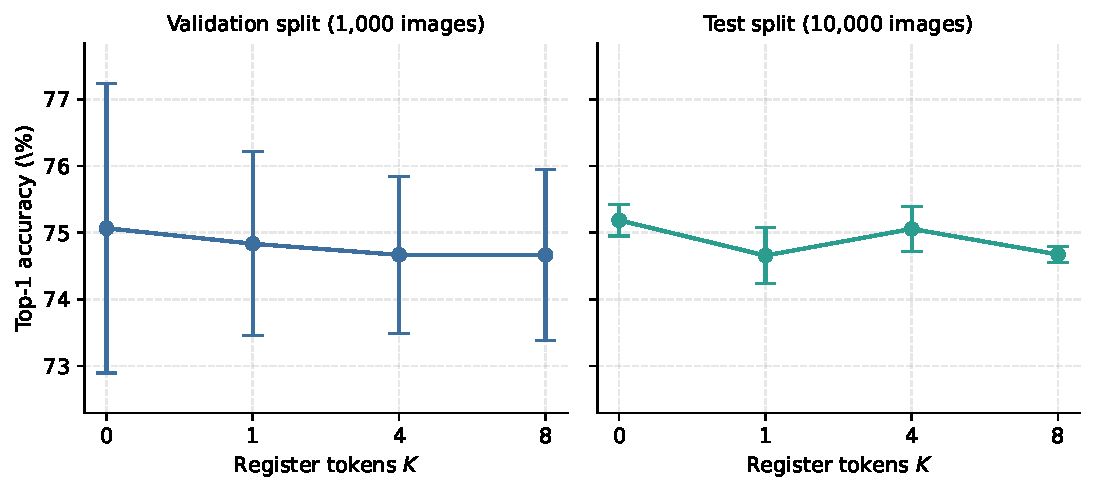
\includegraphics[width=\columnwidth]{accuracy_vs_registers.pdf}
\caption{Top-1 accuracy against register count on the two evaluation splits,
drawn on a shared vertical range. The validation panel is nearly uninformative
at this sample size; the test panel, on ten times the data, resolves the arms
and places the control first.}
\label{fig:accuracy}
\end{figure}

\subsection{H2: the $K=8$ arm degrades, consistent with capacity dilution}

$K=8$ is the one arm with a statistically consistent negative effect on
held-out data. Its paired test-loss difference is $+0.0203$ with the same sign
in 3 of 3 seeds, $t = 8.37$, $p = 0.014$---the smallest $p$-value in the study,
and the only one below $0.05$ on a test-split quantity. It also has the lowest
Top-5 accuracy of the four arms and the lowest final-block attention entropy,
the latter falling in 3 of 3 seeds ($\bar{\delta} = -0.0971$, $p = 0.066$). Its
Top-1 accuracy is not the lowest: $K=1$ is marginally worse
($74.66\%$ against $74.67\%$), a gap far inside the seed noise, so on Top-1 the
two arms are tied for last rather than ordered.

The accuracy response across $K$ is non-monotonic, as H2 predicts: it drops at
$K=1$, partially recovers at $K=4$, and drops again at $K=8$. We report the
non-monotonicity because it is what the hypothesis names, but with three seeds
per arm and a total range of $0.53$ pp we do not claim the shape of the curve is
resolved. What is resolved is the endpoint: eight registers on a $d = 192$
backbone are measurably worse than none.

\subsection{H3: no entropy-collapse effect}

\begin{figure}[t]
\centering

\includegraphics[width=\columnwidth]{entropy_vs_layer.pdf}
\caption{Layer-wise attention entropy. Left: absolute entropy per block, with
$\pm 1\sigma$ bands over seeds; the four arms are visually indistinguishable.
Right: the paired per-seed difference from the control, which is the only view
in which effects of this size are legible.}
\label{fig:entropy}
\end{figure}

Fig.~\ref{fig:entropy} shows the layer profile. Entropy is strongly
depth-dependent and non-monotonic---a minimum of $3.34$ bits at block 2, a
maximum of $6.27$ bits at block 5, and a decline through the final third---but
that profile is a property of the pretrained backbone, not of the treatment: the
four arms lie on top of one another. Averaged over all twelve blocks the paired
differences are $+0.020$, $+0.001$ and $-0.025$ bits for $K = 1, 4, 8$, none
significant. Registers do lower entropy in block 1 (by $0.19$ bits at $K=8$,
$0.12$ at $K=4$, $0.07$ at $K=1$) and raise it in blocks 9 and 11 at
$K \in \{1,4\}$ (largest: $+0.15$ bits at $K=1$, block 9), but no arm shows the deep-layer
entropy \emph{rise} relative to control that H3 requires. The one consistent
deep-layer effect runs the wrong way: $K=8$ lowers block-12 entropy in every
seed.

The patch-norm outlier rate agrees. Averaged over blocks it is
$1.227\%$, $1.246\%$, $1.250\%$ and $1.254\%$ for $K = 0, 1, 4, 8$. The paired
differences are positive for every register arm---the artifact rate rises
slightly rather than falling---though none approaches significance
($p = 0.24$ to $0.53$). We therefore find no evidence for the artifact-removal
mechanism in this regime, in either the entropy or the outlier readout.

\subsection{Optimisation behaviour}

\begin{figure}[t]
\centering

\includegraphics[width=\columnwidth]{loss_curves.pdf}
\caption{Seed-averaged loss trajectories, $\pm 1\sigma$ bands. Training curves
are superimposed across arms; validation curves are dominated by the noise of a
1{,}000-image split.}
\label{fig:curves}
\end{figure}

Fig.~\ref{fig:curves} confirms that the arms are not distinguishable during
optimisation either. The training trajectories coincide from the first epoch,
which is the expected consequence of adding at most 1{,}536 parameters to a
5.54\,M-parameter model. Validation trajectories are visibly noisy and cross
repeatedly. Best epochs cluster late---means of $49.0$, $47.3$, $49.0$ and
$44.7$ for $K = 0, 1, 4, 8$---so no arm was still improving materially at the
budget boundary, and the $K=8$ arm's earlier mean best epoch is consistent with
it having less to gain from the remaining schedule.

\section{Discussion}
\label{sec:discussion}

\subsection{Why the effect appears on one split and not the other}

The most useful insight this experiment produced is a clean instance of a common
failure mode. Had we reported validation loss and the generalization gap, the
two quantities our hypotheses were literally stated on, we would have
concluded that four register tokens regularize a data-starved ViT-Tiny, with a
consistent direction in every seed and $p = 0.024$. The test split demonstrates
otherwise, and it does so unambiguously: the same arm's test-loss difference is
$+0.002$ with $p = 0.823$.

Three properties of the setup explain the dissociation. The validation split
holds 1{,}000 images, one tenth of the test split, and its between-seed
dispersion is nine times larger. The same split is used to choose the
checkpoint, so the reported validation loss is a minimum over 50 epochs of a
noisy sequence, and anything that changes the shape of that sequence changes its
minimum without necessarily changing the model's quality. And the training loss
does not move at all across arms, which removes the mechanism a genuine regularizer
would have to act through: there is no trade of training fit for validation fit
here, only a different draw from the same distribution. Furthermore, scaling the
training budget to 300 images per class confirms that this dissociation is not
simply an artifact of extreme starvation: when overall performance scales by
$+6.14\%$, the held-out null result persists intact.

We draw a methodological conclusion from this rather than only a negative
empirical one. In small-data ablations, a generalization-gap argument built on a
validation split that also performs model selection is not evidence of
generalization. The gap should be reported, as we do, but the claim has to be
settled on held-out data that played no role in checkpoint selection.

\subsection{Why registers may not transfer to this regime}

Our result does not contradict \cite{darcet2024registers}; it bounds where that
mechanism applies. Four differences separate the regimes.

\textbf{Pretraining mismatch.} Our backbone is ImageNet-pretrained and its
registers are not. The pretrained weights encode 12 blocks of routing behaviour
learned in a sequence that had no register positions in it, and the model is
then given 50 epochs over 9{,}000 images to discover that a new set of tokens is
available as scratch space. In \cite{darcet2024registers} the registers are
present throughout pretraining, over datasets larger by three to four orders of
magnitude. It would be surprising if a routing convention learned over hundreds
of millions of images reorganised itself in this budget, and our entropy
measurements indicate it did not: the layer-wise profile of every register arm
is the pretrained profile.

\textbf{The artifacts are present but unmoved.} Our control arm shows a
patch-norm outlier rate of $1.23\%$, about $2.4$ of 196 patches per image. That
is roughly nine times the $0.13\%$ a three-sigma threshold would select from
Gaussian norms, so the heavy-tailed structure the artifact metric is designed to
detect is genuinely there. What is absent is any response to the treatment: the
rate is $1.25\%$ at $K=8$, and the paired differences are positive for every
register arm. The intervention that was introduced to absorb this structure does
not measurably absorb it here, which is a stronger negative statement than
``there was nothing to remove''.

\textbf{Capacity.} At $d = 192$ with 3 heads, eight registers occupy $4\%$ of a
205-token sequence and compete for the same softmax mass as 196 patches. The
$K=8$ degradation we measure is small but is the study's most statistically
consistent effect on held-out data, and it is the direction H2 predicts.

\textbf{Sequence-level dilution, not parameter count.} It is worth being precise
about the mechanism H2 names. Registers add 1{,}536 parameters at $K=8$; no
plausible capacity argument runs through that number. The dilution, if it is
real, is in the attention distribution rather than in the weights: every query
row must now allocate probability across $K$ additional keys that carry no image
content, and at $d = 192$ the model has little margin to spare.

\subsection{What a positive result would have required}

If registers regularize, the signature should be a training loss that rises
while held-out loss falls. We observe neither. A future test with a real chance
of detecting the effect would pretrain with the registers in place, or fine-tune
long enough for the routing to reorganise, or start from a regime where the
artifact rate is measurably elevated in the first place. Absent one of those
changes, adding register tokens to a pretrained small ViT and fine-tuning on
scarce data is, on this evidence, a no-op at best.

\subsection{An exploratory check: registers without training}

The negative result above concerns registers introduced via fine-tuning. A
separate mechanism, proposed independently of our study, avoids training
entirely: Jiang et al.~\cite{jiang2025} identify the specific neurons
responsible for high-norm outlier tokens and redirect their activity into an
untrained token slot at inference time, with no gradient updates. We ran a
small, exploratory check of this idea against our own $K=0$ checkpoints, using
a simplified single-block reimplementation rather than a full port of their
method.

Three conditions were tested across the same three $K=0$ checkpoints (seeds
42, 1337, 3407): a passive empty token slot with no redirection ($+0.07$ pp
over baseline), active redirection of four identified neurons at block~1
($+0.064$ pp), and at block~9 ($+0.06$ pp). A fourth condition, redirection at
block~11 (the final block), returned results numerically identical to the
passive-slot condition in every seed. This is not an empirical null finding
but an architectural necessity: block~11 is followed by no further
self-attention, and the classification head reads only the [CLS] token, so
any intervention confined to non-CLS positions at the final block has no path
back to the token the model is evaluated on. We report this as a
methodological note rather than evidence about the register mechanism at
block~11.

Among the two valid targets (blocks~1 and~9), active redirection did not
exceed the passive empty-slot condition, and all differences are far smaller
than the between-seed dispersion of the $K=0$ baseline itself ($0.30$ pp). We
treat this as a small additional data point consistent with our main
conclusion rather than independent confirmatory evidence: this check used a
single block, four neurons, and three seeds, with no paired statistical
treatment matching Table~II, and should not be read with the same confidence
as the primary ablation.

\begin{table}[h]
\centering
\caption{Exploratory test-time register check (no training), $K=0$
checkpoints, three seeds. Block~11 is architecturally incapable of affecting
the CLS-read classification head; see text.}
\label{tab:test_time_registers}
\begin{tabular}{lc}
\toprule
Condition & Test Top-1 (\%) \\
\midrule
Baseline ($K=0$, untouched)         & $75.18 \pm 0.30$ \\
Passive empty slot (no redirection) & $75.25 \pm 0.24$ \\
Redirection at block 1              & $75.25 \pm 0.26$ \\
Redirection at block 9              & $75.24 \pm 0.25$ \\
\bottomrule
\end{tabular}
\end{table}

\section{Limitations}
\label{sec:limitations}

We state the limits of this study plainly, because a negative result is only
useful if the reader can judge how far it generalises.

\textbf{Three seeds.} Every $p$-value here has $\mathrm{df} = 2$. The tests can
detect only large, perfectly consistent effects, and the fifteen comparisons in
Table~\ref{tab:paired_effects} are uncorrected. We rely on the direction count
as the primary signal for this reason, and we do not claim that any effect we
failed to detect is absent---only that it is smaller than this design can see.

\textbf{One architecture, one dataset, one budget.} The result is established
for ViT-Tiny at $d = 192$, on a 100-image-per-class CIFAR-100 subset, for 50
epochs from ImageNet-pretrained weights. It says nothing about ViT-Small or
larger, about datasets whose statistics differ from CIFAR-100, or about longer
schedules.

\textbf{Pretrained initialisation.} This is the most consequential limitation.
Registers were introduced as a pretraining-time intervention and we apply them
at fine-tuning time. Our result therefore bounds the fine-tuning use of
registers, not the mechanism itself. A from-scratch replication at this scale
would test the original claim more directly and is the obvious next experiment.

\textbf{Diagnostics from 64 images.} Entropy and outlier rates are computed on
the first test batch only. The batch is identical across all twelve runs, so the
paired comparison is sound, but the absolute values are estimates from 64
images and their standard deviations reflect seed variation rather than sampling
variation over the test set. A full-split diagnostic pass would tighten
Fig.~\ref{fig:entropy}; it was not run because the hooks materialise the
$[B,H,S,S]$ attention tensor and doing so over 10{,}000 images did not fit the
project's memory and time budget.

\textbf{Entropy is averaged over all queries.} Our $\bar{H}^{(l)}$ averages over
every query row, whereas the artifact phenomenon is described primarily for the
\texttt{[CLS]} query. A \texttt{[CLS]}-restricted entropy is a sharper
instrument for H3 and would be the first refinement to make; the qualitative
attention maps we generate use exactly that row, but we did not reduce them to
a scalar diagnostic.

\textbf{Validation-based selection.} Checkpoints are chosen on the same
1{,}000-image split whose loss we then report. We treat this as a finding rather
than only a flaw---it is what produces the dissociation of
Section~\ref{sec:discussion}---but it does mean our validation numbers are
selected extrema and should not be read as unbiased estimates.

\section{Conclusion}

We asked whether register tokens regularize a vision transformer when data is
scarce, and answered it with a fully paired 24-run controlled ablation across two
distinct data regimes (100 and 300 images per class) in which the register count
was the strictly isolated variable. The answer is no. No register configuration
improves held-out Top-1 accuracy over the register-free baseline ($75.19 \pm 0.24\%$
at 100 images/class and $81.33 \pm 0.37\%$ at 300 images/class). While tripling the
training budget provides a clear $+6.14\%$ accuracy gain, registers confer no
advantage over control in either regime ($p > 0.50$), confirming that the empirical
null result is scale-invariant across low-data regimes.

The study's more transferable methodological result is how nearly an uncareful
protocol would have concluded the opposite. On the 100-image/class validation split,
$K=4$ narrows the generalization gap in every seed and lowers validation loss in
every seed at $p = 0.024$, presenting what initially appears to be a textbook
regularization signature. Crucially, this effect completely vanishes on the held-out
test split ($p = 0.823$). The training loss, invariant across all four arms to within
$0.005$ nats, reveals the mechanism: nothing was traded during optimization, so
nothing was regularized. A generalization gap measured on the very split used for
model selection does not constitute evidence of generalization.

At $K=8$, we find the single consistent held-out effect in the low-data regime, and
it is a penalty: test loss degrades across all three seeds ($p = 0.014$) and
final-block attention entropy declines in all three. On a 192-dimensional backbone,
allocating eight tokens that carry no visual content imposes a measurable capacity cost.

We view this as a scope result rather than a refutation of the register mechanism.
Registers were introduced as a pretraining-time intervention at foundation scale;
we applied them at fine-tuning time to a compact pretrained model under constrained
data budgets. Mechanistic attention diagnostics confirm that pretrained routing does
not reorganize to exploit registers in low-data regimes. The definitive experiment to
distinguish whether registers do not help in small models or whether they cannot be
added post-hoc is a from-scratch replication at this scale, and our open sweep
infrastructure executes that evaluation without modification.


\section*{Reproducibility}
The training code, the sweep runner, the aggregation engine and the scripts that
generate every table and figure in this paper are available at
\url{https://github.com/shahin1717/vit-research}. Table~\ref{tab:main_results}
and Table~\ref{tab:paired_effects} are emitted by
\texttt{src/utils/export\_latex.py} directly from
\texttt{outputs/sweep\_summary.json}; the figures are emitted by
\texttt{scripts/plot\_metrics.py} from the same artifact. No number in this
paper was transcribed by hand.

\bibliographystyle{IEEEtran}
\bibliography{refs}

\end{document}
